\chapter{Functions, Procedures, and Co-Expressions}

\textsc{Perspective}: The invocation of functions and procedures is
central to the evaluation of expressions in most programming
languages. In Icon, this activity has several aspects that complicate
its implementation. Functions and procedures are data values that can
be assigned to identifiers, passed as arguments, and so
on. Consequently, the meaning of an invocation expression cannot be
determined until it is evaluated. Functions and procedures can be
called with more or fewer arguments than expected. Thus, there must be
a provision for adjusting argument lists at run time.  Since mutual
evaluation has the same syntax as function and procedure invocation,
run-time processing of such expressions is further complicated.

Co-expressions, which require separate stacks for their evaluation,
add complexities and dependencies on computer architecture that are
not found elsewhere in the implementation.

\section[10.1 Invocation Expressions]{10.1 Invocation Expressions}

As mentioned in Sec. 8.2.4, the virtual machine code for an expression such as

%-% {\ttfamily\mdseries
%-% \textit{\ \ \ expr0(expr1, expr2, }..., \textit{exprn)}}
\iconline{ \textit{\ \ \ expr0(expr1, expr2, }..., \textit{exprn)} }

\noindent is

%-% {\ttfamily\mdseries
%-% \ \ \ code for expr0}
%-% 
%-% {\ttfamily\mdseries
%-% \ \ \ code for expr1}
%-% 
%-% {\ttfamily\mdseries
%-% \ \ \ code for expr2}
%-% 
%-% {\ttfamily\mdseries
%-% \ \ \ ...}
%-% 
%-% {\ttfamily\itshape
%-% \ \ \ code for exprn}
%-% 
%-% {\ttfamily
%-% \ \ \ invoke n}
\goodbreak
\iconcode{
\>code for expr0\\
\>code for expr1\\
\>code for expr2\\
\>...\\
\>code for exprn\\
\>invoke n
}

Consequently, the stack when the \texttt{invoke} instruction is executed is

\begin{center}
%--%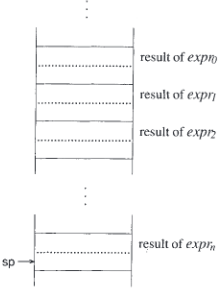
\includegraphics[width=2.19in,height=2.88in]{ib-img/invokestack.png}
\begin{picture}(300,200)(0,16)
\put(100,32){\dvbox{}{}{}}
\put(100,32){\lregptr{sp}{20}}
\put(100,32){\trboxlabel{result of \textit{expr\TextSubscript{n}}}}
\put(100,32){\downbars}
\put(100,32){\upetc}
\put(100,112){\downetc}
\put(100,112){\dvbox{}{}{}}
\put(100,112){\trboxlabel{result of \textit{expr\TextSubscript{2}}}}
\put(100,144){\dvbox{}{}{}}
\put(100,144){\trboxlabel{result of \textit{expr\TextSubscript{1}}}}
\put(100,176){\dvbox{}{}{}}
\put(100,176){\trboxlabel{result of \textit{expr\TextSubscript{0}}}}
\put(100,176){\upetc}
\end{picture}
\end{center}

The meaning of the expression, and hence the action taken by
\texttt{invoke}, depends on the result produced by
\textit{expr\TextSubscript{0}}. If the value of
\textit{expr\TextSubscript{0}} is an integer or convertible to an
integer, the invocation expression corresponds to mutual
evaluation. If this integer is negative, it is converted to the
corresponding positive value with respect to the number of arguments,
If the value is between one and n, the corresponding descriptor is
copied on top of the result of \textit{expr\TextSubscript{0}},
\texttt{sp} is set to this position, and \texttt{invoke} transfers
control to the beginning of the interpretive loop. On the other hand,
if the value is out of range, \texttt{invoke} fails. Note that the
returned value overwrites the descriptor for
\textit{expr\TextSubscript{0}}, whereas for operators a null-valued
descriptor is pushed to receive the value.

If the value of \textit{expr\TextSubscript{0}} is a function or a
procedure, the corresponding function or procedure must be invoked
with the appropriate arguments. A function or procedure value is
represented by a descriptor that points to a block that contains
information about the function or procedure.

\section[10.2 Procedure Blocks]{10.2 Procedure Blocks}

Functions and procedures have similar blocks, and there is no
source-language type distinction between them.

\textbf{Blocks for Procedures. }Blocks for procedures are constructed
by the linker, using information provided by the translator. Such
blocks are read in as part of the icode file when an Icon program is
executed. The block for a procedure contains the usual title and size
words, followed by six words that characterize the procedure:

\liststyleLxi
\begin{enumerate}
\item 
The icode location of the first virtual machine instruction for the procedure.
\item 
\ The number of arguments expected by the procedure.
\item 
\ The number of local identifiers in the procedure.
\item 
\ The number of static identifiers in the procedure.
\item 
The index in the static identifier array of the first
static identifier in the procedure.
\item 
A C string for the name of the file in which the procedure
declaration occurred.
\end{enumerate}

The remainder of the procedure block contains qualifiers: one for the
string name of the procedure, then others for the string names of the
arguments, local identifiers, and static identifiers, in that order.


For example, the procedure declaration

%-% {\ttfamily\mdseries
%-% \ \ \ procedure calc(i,j)}
%-% 
%-% {\ttfamily\mdseries
%-% \ \ \ local k}
%-% 
%-% {\ttfamily\mdseries
%-% \ \ \ static base, index}
%-% 
%-% {\ttfamily\mdseries
%-% \ \ \ \ \ \ \ \ \ \ \ .}
%-% 
%-% {\ttfamily\mdseries
%-% \ \ \ \ \ \ \ \ \ \ \ .}
%-% 
%-% {\ttfamily\mdseries
%-% \ \ \ \ \ \ \ \ \ \ \ .}
%-% 
%-% {\ttfamily\mdseries
%-% \ \ \ end}
\goodbreak
\iconcode{
\>procedure calc(i,j)\\
\>local k\\
\>static base, index\\
\>\>\>\ \ \vdots\\
\>end
}

\noindent has the following procedure block:

%--%\ \  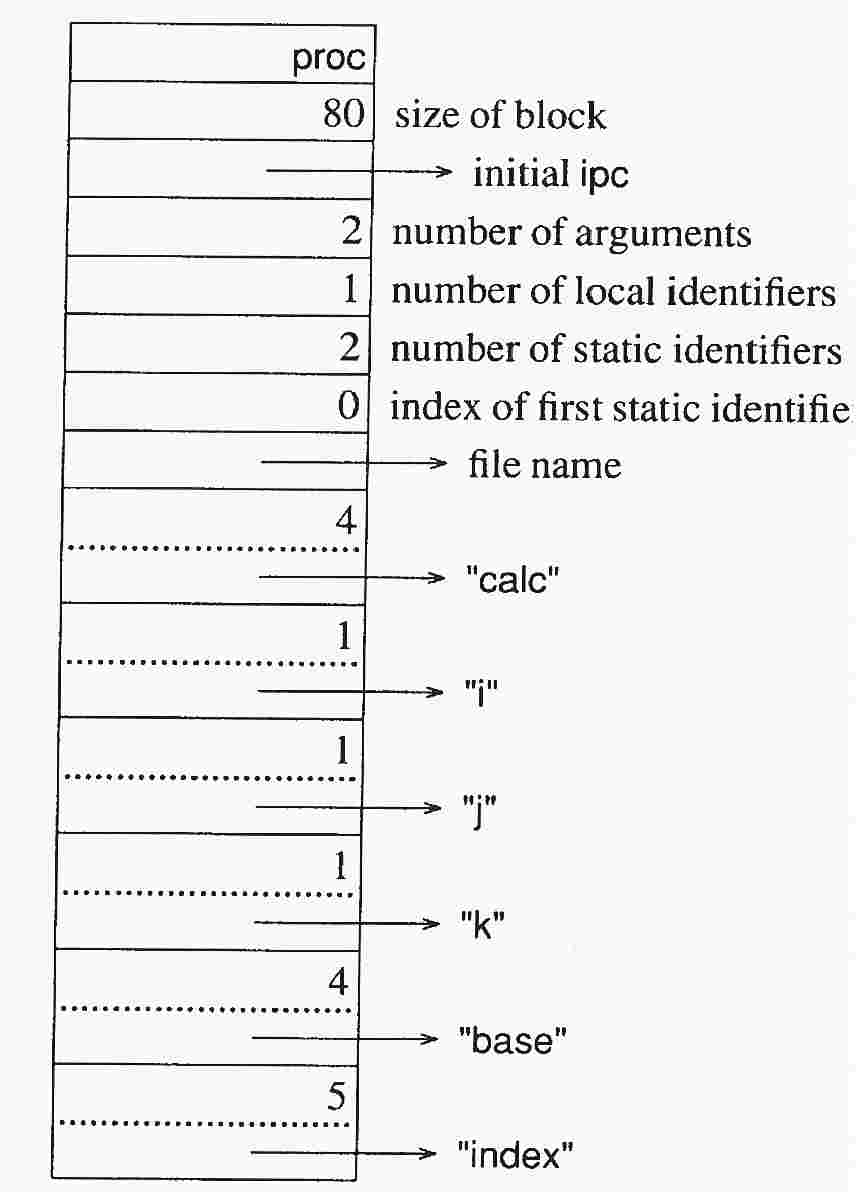
\includegraphics[width=2.8846in,height=3.9807in]{ib-img/ib-img077.jpg} 
\begin{picture}(300,340)
\begin{picture}(0,0)(-100,-192)
\put(0,0){\blkptrbox{0}{40}{file name}}
\put(0,0){\trboxlabel{index of first static identifier}}
\put(0,32){\blkbox{1}{2}}
\put(0,32){\rightboxlabels{number of local identifiers}{number of static identifiers}}
\put(0,64){\wordbox{2}{}}
\put(0,64){\brboxlabel{number of arguments}}
\put(0,80){\blkptrbox{80}{40}{initial ipc}}
\put(0,80){\trboxlabel{size of block}}
\put(0,112){\wordbox{proc}{}}
\end{picture}
\put(100,0){\dvptrbox{5}{}{40}{"index"}}
\put(100,32){\dvptrbox{4}{}{40}{"base"}}
\put(100,64){\dvptrbox{1}{}{40}{"k"}}
\put(100,96){\dvptrbox{1}{}{40}{"j"}}
\put(100,128){\dvptrbox{1}{}{40}{"i"}}
\put(100,160){\dvptrbox{4}{}{40}{"calc"}}
\end{picture}

The 0 value for the index in the static identifier array indicates
that base is the first static identifier in the program. The indices
of static identifiers are zero-based and increase throughout a program
as static declarations occur.


\textbf{Blocks for Functions.} Blocks for functions are created by the
macro FncDcl that occurs at the beginning of every C function that
implements an Icon function. Such blocks for functions are similar to
those for procedures but are distinguished by the value -1 in the word
that otherwise contains the number of local identifiers. The entry
point is the entry point of the C routine for the function. The
procedure block for \texttt{repl} is typical:


%--%\ \  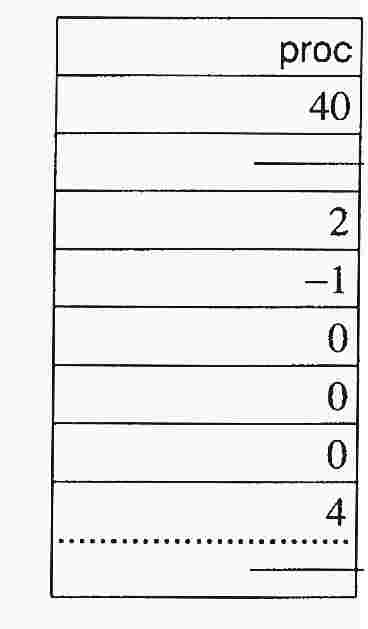
\includegraphics[width=1.2819in,height=2.1008in]{ib-img/ib-img078.jpg} 
\begin{picture}(300,170)
\begin{picture}(0,0)(-100,-32)
\put(0,0){\blkbox{0}{0}}
\put(0,0){\rightboxlabels{not used}{not used}}
\put(0,32){\blkbox{-1}{0}}
\put(0,32){\rightboxlabels{function indicator}{not used}}
\put(0,64){\wordbox{2}{}}
\put(0,64){\brboxlabel{number of arguments}}
\put(0,80){\blkptrbox{40}{40}{C entry point}}
\put(0,80){\trboxlabel{size of block}}
\put(0,112){\wordbox{proc}{}}
\end{picture}
\put(100,0){\dvptrbox{4}{}{40}{"repl"}}
\end{picture}

\noindent Note that there are no argument names.

Some functions, such as \texttt{write()}, allow an arbitrary number of
arguments. This is indicated by the value -1 in place of the number of
arguments:


%--%\ \  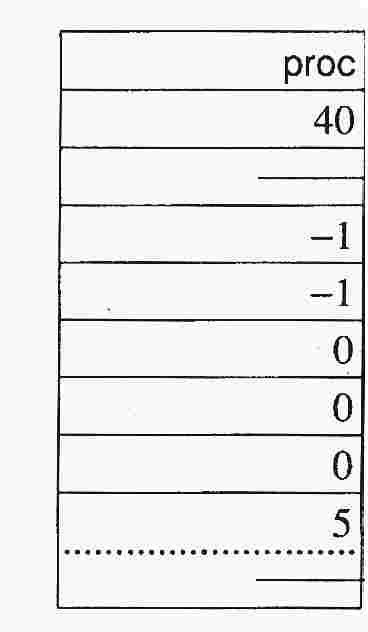
\includegraphics[width=1.2819in,height=2.1098in]{ib-img/ib-img079.jpg} 
\begin{picture}(300,170)
\begin{picture}(0,0)(-100,-32)
\put(0,0){\blkbox{0}{0}}
\put(0,0){\rightboxlabels{not used}{not used}}
\put(0,32){\blkbox{-1}{0}}
\put(0,32){\rightboxlabels{function indicator}{not used}}
\put(0,64){\wordbox{-1}{}}
\put(0,64){\brboxlabel{indicator of a variable number of arguments}}
\put(0,80){\blkptrbox{40}{40}{C entry point}}
\put(0,80){\trboxlabel{size of block}}
\put(0,112){\wordbox{proc}{}}
\end{picture}
\put(100,0){\dvptrbox{5}{}{40}{"write"}}
\end{picture}

\section[10.3 Invocation]{10.3 Invocation}
\subsection[10.3.1 Argument Processing]{10.3.1 Argument Processing}

Argument processing begins by dereferencing the arguments in place on
the stack. If a fixed number of arguments is specified in the
procedure block, this number is compared with the argument of
\texttt{invoke}, which is the number of arguments on the stack.


If there are too many arguments, \texttt{sp} is set to point to the
last one expected. For example, the expression

%-% {\ttfamily\mdseries
%-% \ \ numeric(i, j)}
\iconline{ \ \ numeric(i, j) }

\noindent results in

%--%\ \  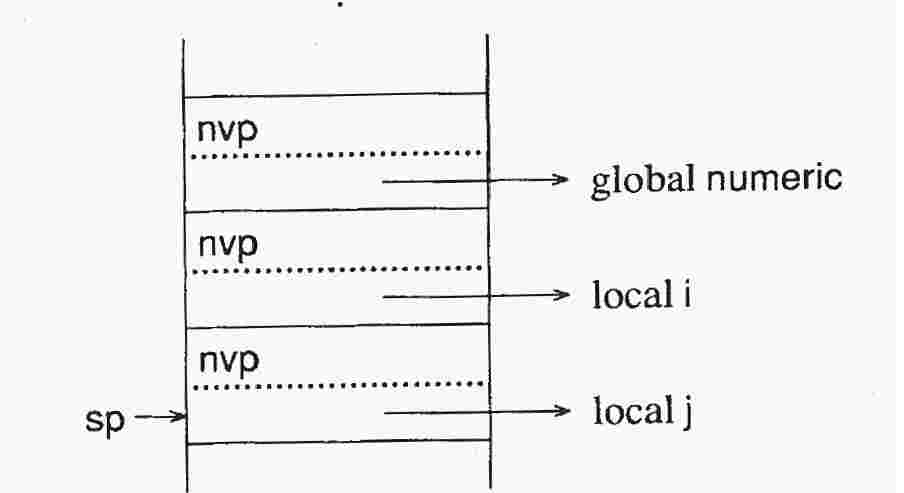
\includegraphics[width=3.0984in,height=1.6457in]{ib-img/ib-img080.jpg} 
\begin{picture}(300,130)(0,-16)
\put(100,0){\downbars}
\put(100,0){\lregptr{sp}{20}}
\put(100,0){\dvptrbox{}{nvp}{40}{local j}}
\put(100,32){\dvptrbox{}{nvp}{40}{local i}}
\put(100,64){\dvptrbox{}{nvp}{40}{global numeric}}
\put(100,64){\upetc}
\end{picture}

\noindent Since \texttt{numeric()} expects only one argument, \texttt{sp} is reset, 
effectively popping the second argument:

%--%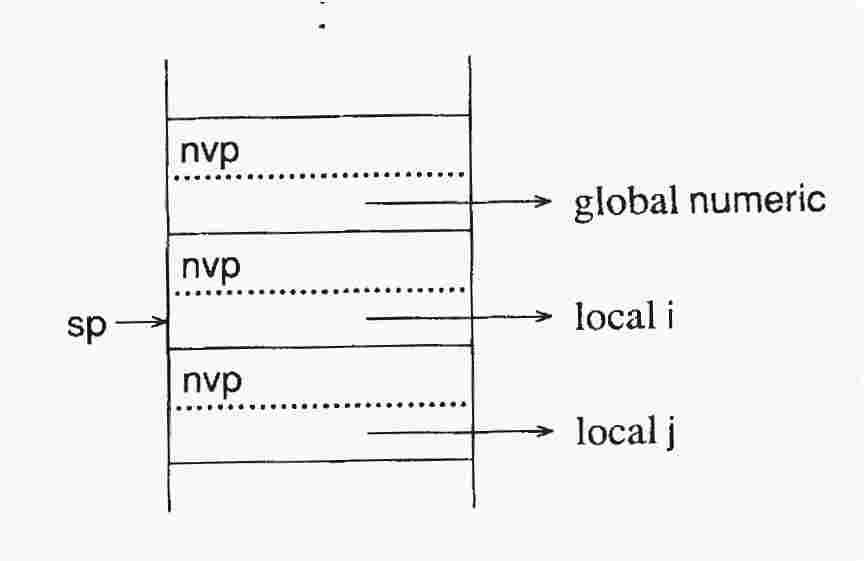
\includegraphics[width=2.8846in,height=1.8728in]{ib-img/ib-img081.jpg} 
\begin{picture}(300,130)(0,-16)
\put(100,0){\downbars}
\put(100,32){\lregptr{sp}{20}}
\put(100,0){\dvptrbox{}{nvp}{40}{local j}}
\put(100,32){\dvptrbox{}{nvp}{40}{local i}}
\put(100,64){\dvptrbox{}{nvp}{40}{global numeric}}
\put(100,64){\upetc}
\end{picture}

\noindent On the other hand, if there are not enough arguments, null-valued
descriptors pushed to supply the missing arguments.  For example, the
expression

%-% {\ttfamily\mdseries
%-% \ \ left(s, i)}
\iconline{ \ \ left(s, i) }

\noindent results in

%--%\ \  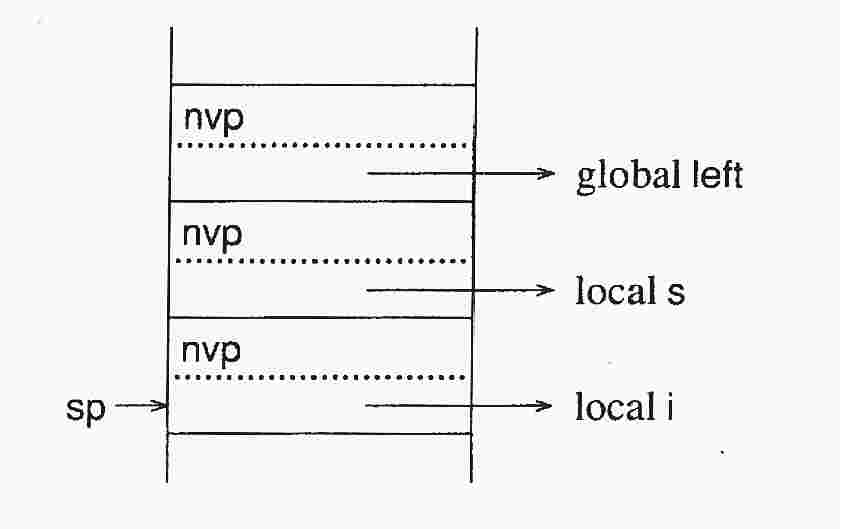
\includegraphics[width=2.8846in,height=1.7661in]{ib-img/ib-img082.jpg} 
\begin{picture}(300,130)(0,-16)
\put(100,0){\downbars}
\put(100,0){\lregptr{sp}{20}}
\put(100,0){\dvptrbox{}{nvp}{40}{local i}}
\put(100,32){\dvptrbox{}{nvp}{40}{local s}}
\put(100,64){\dvptrbox{}{nvp}{40}{global left}}
\put(100,64){\upetc}
\end{picture}

\noindent and a null value is pushed to provide the missing third argument:

%--%\ \  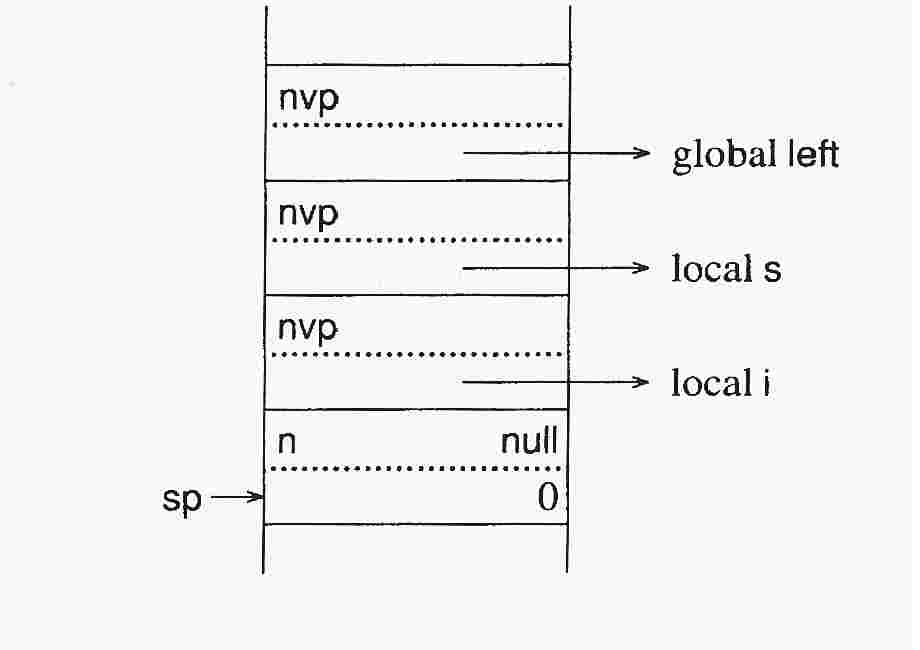
\includegraphics[width=3.0984in,height=2.1701in]{ib-img/ib-img083.jpg} 
\begin{picture}(300,160)(0,-16)
\begin{picture}(0,0)(0,-32)
\put(100,0){\dvptrbox{}{nvp}{40}{local i}}
\put(100,32){\dvptrbox{}{nvp}{40}{local s}}
\put(100,64){\dvptrbox{}{nvp}{40}{global left}}
\put(100,64){\upetc}
\end{picture}
\put(100,0){\downbars}
\put(100,0){\dvbox{null}{n}{0}}
\put(100,0){\lregptr{sp}{20}}
\end{picture}

\subsection[10.3.2 Function Invocation]{10.3.2 Function Invocation}

Function invocation involves calling a C function in a fashion that is
very similar to evaluating an operator. In the case of an Icon
function, the entry point of the corresponding C function is obtained
from the procedure block rather than by indexing an array of function
pointers corresponding to operator codes.

For an Icon function that has a fixed number of arguments, the C
function is called with a single argument that is a pointer to the
location of Arg0 on the interpreter stack. Note that Arg0 is the
descriptor that points to the procedure block. For an Icon function
that may be called with an arbitrary number of arguments, the C
function is called with two arguments: the number of arguments on the
stack and a pointer to Arg0.

Like an operator, a function may fail, return a result, or
suspend. The coding protocol is the same as for operators.  The
function find is an example:

%-% {\ttfamily\mdseries
%-% function\{*\} find(s1,s2,i,j)}
%-% 
%-% {\ttfamily\mdseries
%-% \ \ \ str\_anal( s2, i, j )}
%-% 
%-% {\ttfamily\mdseries
%-% \ \ \ if !cnv:string(s1) then}
%-% 
%-% {\ttfamily\mdseries
%-% \ \ \ \ \ \ runerr(103,s1)}
%-% 
%-% {\ttfamily\mdseries
%-% \ \ \ body \{}
%-% 
%-% {\ttfamily\mdseries
%-% \ \ \ \ \ \ register char *str1, *str2;}
%-% 
%-% {\ttfamily\mdseries
%-% \ \ \ \ \ \ C\_integer s1\_len, l, term;}
%-% 
%-% 
%-% \bigskip
%-% 
%-% {\ttfamily\mdseries
%-% \ \ \ \ \ \ /*}
%-% 
%-% {\ttfamily\mdseries
%-% \ \ \ \ \ \ \ * Loop through s2[i:j] trying to find s1 at each point,}
%-% 
%-% {\ttfamily\mdseries
%-% \ \ \ \ \ \ \ * stopping when the remaining portion s2[i:j] is too short}
%-% 
%-% {\ttfamily\mdseries
%-% \ \ \ \ \ \ \ * to contain s1. Optimize me!}
%-% 
%-% {\ttfamily\mdseries
%-% \ \ \ \ \ \ \ */}
%-% 
%-% {\ttfamily\mdseries
%-% \ \ \ \ \ \ s1\_len = StrLen(s1);}
%-% 
%-% {\ttfamily\mdseries
%-% \ \ \ \ \ \ term = cnv\_j - s1\_len;}
%-% 
%-% {\ttfamily\mdseries
%-% \ \ \ \ \ \ while (cnv\_i {\textless}= term) \{}
%-% 
%-% {\ttfamily\mdseries
%-% \ \ \ \ \ \ \ \ \ str1 = StrLoc(s1);}
%-% 
%-% {\ttfamily\mdseries
%-% \ \ \ \ \ \ \ \ \ str2 = StrLoc(s2) + cnv\_i - 1;}
%-% 
%-% {\ttfamily\mdseries
%-% \ \ \ \ \ \ \ \ \ l \ \ \ = s1\_len;}
%-% 
%-% 
%-% \bigskip
%-% 
%-% {\ttfamily\mdseries
%-% \ \ \ \ \ \ \ \ \ /*}
%-% 
%-% {\ttfamily\mdseries
%-% \ \ \ \ \ \ \ \ \ \ * Compare strings on a byte-wise basis; if the end is}
%-% 
%-% {\ttfamily\mdseries
%-% \ \ \ \ \ \ \ \ \ \ * reached before inequality is found, suspend with the}
%-% 
%-% {\ttfamily\mdseries
%-% \ \ \ \ \ \ \ \ \ \ * position of the string.}
%-% 
%-% {\ttfamily\mdseries
%-% \ \ \ \ \ \ \ \ \ \ */}
%-% 
%-% {\ttfamily\mdseries
%-% \ \ \ \ \ \ \ \ \ do \{}
%-% 
%-% {\ttfamily\mdseries
%-% \ \ \ \ \ \ \ \ \ \ \ \ if (l-{}- {\textless}= 0) \{}
%-% 
%-% {\ttfamily\mdseries
%-% \ \ \ \ \ \ \ \ \ \ \ \ \ \ \ suspend C\_integer cnv\_i;}
%-% 
%-% {\ttfamily\mdseries
%-% \ \ \ \ \ \ \ \ \ \ \ \ \ \ \ break;}
%-% 
%-% {\ttfamily\mdseries
%-% \ \ \ \ \ \ \ \ \ \ \ \ \ \ \ \}}
%-% 
%-% {\ttfamily\mdseries
%-% \ \ \ \ \ \ \ \ \ \ \ \ \} while (*str1++ == *str2++);}
%-% 
%-% {\ttfamily\mdseries
%-% \ \ \ \ \ \ \ \ \ cnv\_i++;}
%-% 
%-% {\ttfamily\mdseries
%-% \ \ \ \ \ \ \ \ \ \}}
%-% 
%-% {\ttfamily\mdseries
%-% \ \ \ \ \ \ fail;}
%-% 
%-% {\ttfamily\mdseries
%-% \ \ \ \ \ \ \}}
%-% 
%-% {\ttfamily\mdseries
%-% end}
\goodbreak
\iconcode{
function\{*\} find(s1,s2,i,j)\\
\>str\_anal( s2, i, j )\\
\>if !cnv:string(s1) then\\
\>\>runerr(103,s1)\\
\>body \{\\
\>\>register char *str1, *str2;\\
\>\>C\_integer s1\_len, l, term;\\
\\
\>\>/*\\
\>\>\ * Loop through s2[i:j] trying to find s1 at each point,\\
\>\>\ * stopping when the remaining portion s2[i:j] is too short\\
\>\>\ * to contain s1. Optimize me!\\
\>\>\ */\\
\>\>s1\_len = StrLen(s1);\\
\>\>term = cnv\_j - s1\_len;\\
\>\>while (cnv\_i <= term) \{\\
\>\>\>str1 = StrLoc(s1);\\
\>\>\>str2 = StrLoc(s2) + cnv\_i - 1;\\
\>\>\>l \ \ \ = s1\_len;\\
\\
\>\>\>/*\\
\>\>\>\ * Compare strings on a byte-wise basis; if the end is\\
\>\>\>\ * reached before inequality is found, suspend with the\\
\>\>\>\ * position of the string.\\
\>\>\>\ */\\
\>\>\>do \{\\
\>\>\>\>if (l-{}- <= 0) \{\\
\>\>\>\>\>suspend C\_integer cnv\_i;\\
\>\>\>\>\>break;\\
\>\>\>\>\>\}\\
\>\>\>\>\} while (*str1++ == *str2++);\\
\>\>\>cnv\_i++;\\
\>\>\>\}\\
\>\>fail;\\
\>\>\}\\
end
}

\texttt{str\_anal()} is an RTL multi-line macro for performing the
standard conversions and defaulting for string analysis functions. It
takes as arguments the parameters for subject, beginning position, and
ending position. It produces declarations for these 3 names prepended
with \texttt{cnv\_}. These variables will contain the converted
versions of the arguments.

%-% {\ttfamily\mdseries
%-% \#begdef str\_anal(s, i, j)}
%-% 
%-% {\ttfamily\mdseries
%-% \ \ \ declare \{}
%-% 
%-% {\ttfamily\mdseries
%-% \ \ \ \ \ \ C\_integer cnv\_ \#\# i;}
%-% 
%-% {\ttfamily\mdseries
%-% \ \ \ \ \ \ C\_integer cnv\_ \#\# j;}
%-% 
%-% {\ttfamily\mdseries
%-% \ \ \ \ \ \ \}}
%-% 
%-% 
%-% \bigskip
%-% 
%-% {\ttfamily\mdseries
%-% \ \ \ abstract \{}
%-% 
%-% {\ttfamily\mdseries
%-% \ \ \ \ \ \ return integer}
%-% 
%-% {\ttfamily\mdseries
%-% \ \ \ \ \ \ \}}
%-% 
%-% 
%-% \bigskip
%-% 
%-% {\ttfamily\mdseries
%-% \ \ \ if is:null(s) then \{}
%-% 
%-% {\ttfamily\mdseries
%-% \ \ \ \ \ \ inline \{}
%-% 
%-% {\ttfamily\mdseries
%-% \ \ \ \ \ \ \ \ \ s = k\_subject;}
%-% 
%-% {\ttfamily\mdseries
%-% \ \ \ \ \ \ \ \ \ \}}
%-% 
%-% {\ttfamily\mdseries
%-% \ \ \ \ \ \ if is:null(i) then inline \{}
%-% 
%-% {\ttfamily\mdseries
%-% \ \ \ \ \ \ \ \ \ cnv\_ \#\# i = k\_pos;}
%-% 
%-% {\ttfamily\mdseries
%-% \ \ \ \ \ \ \ \ \ \}}
%-% 
%-% {\ttfamily\mdseries
%-% \ \ \ \ \ \ \}}
%-% 
%-% {\ttfamily\mdseries
%-% \ \ \ else \{}
%-% 
%-% {\ttfamily\mdseries
%-% \ \ \ \ \ \ if !cnv:string(s) then}
%-% 
%-% {\ttfamily\mdseries
%-% \ \ \ \ \ \ \ \ \ runerr(103,s)}
%-% 
%-% {\ttfamily\mdseries
%-% \ \ \ \ \ \ if is:null(i) then inline \{}
%-% 
%-% {\ttfamily\mdseries
%-% \ \ \ \ \ \ \ \ \ cnv\_ \#\# i = 1;}
%-% 
%-% {\ttfamily\mdseries
%-% \ \ \ \ \ \ \ \ \ \}}
%-% 
%-% {\ttfamily\mdseries
%-% \ \ \ \ \ \ \}}
%-% 
%-% 
%-% \bigskip
%-% 
%-% {\ttfamily\mdseries
%-% \ \ \ if !is:null(i) then}
%-% 
%-% {\ttfamily\mdseries
%-% \ \ \ \ \ \ if cnv:C\_integer(i,cnv\_ \#\# i) then inline \{}
%-% 
%-% {\ttfamily\mdseries
%-% \ \ \ \ \ \ \ \ \ if ((cnv\_ \#\# i = cvpos(cnv\_ \#\# i, StrLen(s))) ==}
%-% 
%-% {\ttfamily\mdseries
%-% \ \ \ \ \ \ \ \ \ \ \ \ \ \ CvtFail)}
%-% 
%-% {\ttfamily\mdseries
%-% \ \ \ \ \ \ \ \ \ \ \ \ fail;}
%-% 
%-% {\ttfamily\mdseries
%-% \ \ \ \ \ \ \ \ \ \}}
%-% 
%-% {\ttfamily\mdseries
%-% \ \ \ \ \ \ else}
%-% 
%-% {\ttfamily\mdseries
%-% \ \ \ \ \ \ \ \ \ runerr(101,i)}
%-% 
%-% 
%-% \bigskip
%-% 
%-% {\ttfamily\mdseries
%-% \ \ \ \ if is:null(j) then inline \{}
%-% 
%-% {\ttfamily\mdseries
%-% \ \ \ \ \ \ \ cnv\_ \#\# j = StrLen(s) + 1;}
%-% 
%-% {\ttfamily\mdseries
%-% \ \ \ \ \ \ \ \}}
%-% 
%-% {\ttfamily\mdseries
%-% \ \ \ \ else if cnv:C\_integer(j,cnv\_ \#\# j) then inline \{}
%-% 
%-% {\ttfamily\mdseries
%-% \ \ \ \ \ \ \ if ((cnv\_ \#\# j = cvpos(cnv\_ \#\# j, StrLen(s))) == CvtFail)}
%-% 
%-% {\ttfamily\mdseries
%-% \ \ \ \ \ \ \ \ \ \ fail;}
%-% 
%-% {\ttfamily\mdseries
%-% \ \ \ \ \ \ \ if (cnv\_ \#\# i {\textgreater} cnv\_ \#\# j) \{}
%-% 
%-% {\ttfamily\mdseries
%-% \ \ \ \ \ \ \ \ \ \ register C\_integer tmp;}
%-% 
%-% {\ttfamily\mdseries
%-% \ \ \ \ \ \ \ \ \ \ tmp = cnv\_ \#\# i;}
%-% 
%-% {\ttfamily\mdseries
%-% \ \ \ \ \ \ \ \ \ \ cnv\_ \#\# i = cnv\_ \#\# j;}
%-% 
%-% {\ttfamily\mdseries
%-% \ \ \ \ \ \ \ \ \ \ cnv\_ \#\# j = tmp;}
%-% 
%-% {\ttfamily\mdseries
%-% \ \ \ \ \ \ \ \ \ \ \}}
%-% 
%-% {\ttfamily\mdseries
%-% \ \ \ \ \ \ \ \}}
%-% 
%-% {\ttfamily\mdseries
%-% \ \ \ \ else}
%-% 
%-% {\ttfamily\mdseries
%-% \ \ \ \ \ \ \ runerr(101,j)}
%-% 
%-% {\ttfamily\mdseries
%-% \#enddef}
\goodbreak
\iconcode{
\#begdef str\_anal(s, i, j)\\
\>declare \{\\
\>\>C\_integer cnv\_ \#\# i;\\
\>\>C\_integer cnv\_ \#\# j;\\
\>\>\}\\
\\
\>abstract \{\\
\>\>return integer\\
\>\>\}\\
\\
\>if is:null(s) then \{\\
\>\>inline \{\\
\>\>\>s = k\_subject;\\
\>\>\>\}\\
\>\>if is:null(i) then inline \{\\
\>\>\>cnv\_ \#\# i = k\_pos;\\
\>\>\>\}\\
\>\>\}\\
\>else \{\\
\>\>if !cnv:string(s) then\\
\>\>\>runerr(103,s)\\
\>\>if is:null(i) then inline \{\\
\>\>\>cnv\_ \#\# i = 1;\\
\>\>\>\}\\
\>\>\}\\
\\
\>if !is:null(i) then\\
\>\>if cnv:C\_integer(i,cnv\_ \#\# i) then inline \{\\
\>\>\>if ((cnv\_ \#\# i = cvpos(cnv\_ \#\# i, StrLen(s))) == CvtFail)\\
\>\>\>\>fail;\\
\>\>\>\}\\
\>\>else\\
\>\>\>runerr(101,i)\\
\\
\>\ if is:null(j) then inline \{\\
\>\>\ cnv\_ \#\# j = StrLen(s) + 1;\\
\>\>\ \}\\
\>\ else if cnv:C\_integer(j,cnv\_ \#\# j) then inline \{\\
\>\>\ if ((cnv\_ \#\# j = cvpos(cnv\_ \#\# j, StrLen(s))) == CvtFail)\\
\>\>\>\ fail;\\
\>\>\ if (cnv\_ \#\# i > cnv\_ \#\# j) \{\\
\>\>\>\ register C\_integer tmp;\\
\>\>\>\ tmp = cnv\_ \#\# i;\\
\>\>\>\ cnv\_ \#\# i = cnv\_ \#\# j;\\
\>\>\>\ cnv\_ \#\# j = tmp;\\
\>\>\>\ \}\\
\>\>\ \}\\
\>\ else\\
\>\>\ runerr(101,j)\\
\#enddef
}


\subsection[10.3.3 Procedure Invocation]{10.3.3 Procedure Invocation}

In the case of procedure invocation, a \textit{procedure frame} is
pushed onto the interpreter stack to preserve information that may be
changed during the execution of the procedure and that must be
restored when the procedure returns. As for other types of frames, a
procedure frame begins with a marker. A procedure frame marker
consists of eight words:


%--%\ \  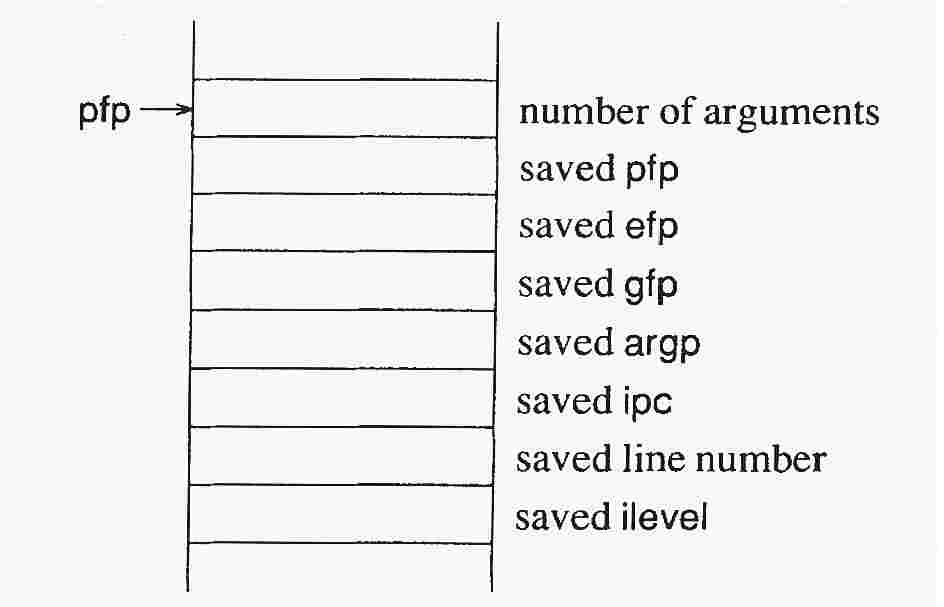
\includegraphics[width=3.2063in,height=2.0272in]{ib-img/ib-img084.jpg} 
\begin{picture}(300,180)(0,-16)
\put(100,0){\downbars}
\put(100,0){\blkbox{}{}}
\put(100,0){\rightboxlabels{saved line number}{saved ilevel}}
\put(100,32){\blkbox{}{}}
\put(100,32){\rightboxlabels{saved argp}{saved ipc}}
\put(100,64){\blkbox{}{}}
\put(100,64){\rightboxlabels{saved efp}{saved gfp}}
\put(100,96){\blkbox{}{}}
\put(100,96){\rightboxlabels{number of arguments}{saved pfp}}
\put(100,96){\upetc}
\put(100,112){\lregptr{pfp}{20}}
\end{picture}

The current procedure frame is pointed to by \texttt{pfp}, and
\texttt{argp} points to the place on the interpreter stack where the
arguments begin, analogous to Arg0 for functions. The number of
arguments, which can be computed from \texttt{pfp} and \texttt{argp},
is provided to make computations related to arguments more convenient.

After the procedure marker is constructed, a null-valued descriptor is
pushed for each local identifier. For example, the call

%-% {\ttfamily\mdseries
%-% \ \ calc(3,4)}
\iconline{ \ \ calc(3,4) }

\noindent for the procedure declaration given in Sec. 10.2 produces

%--%\ \  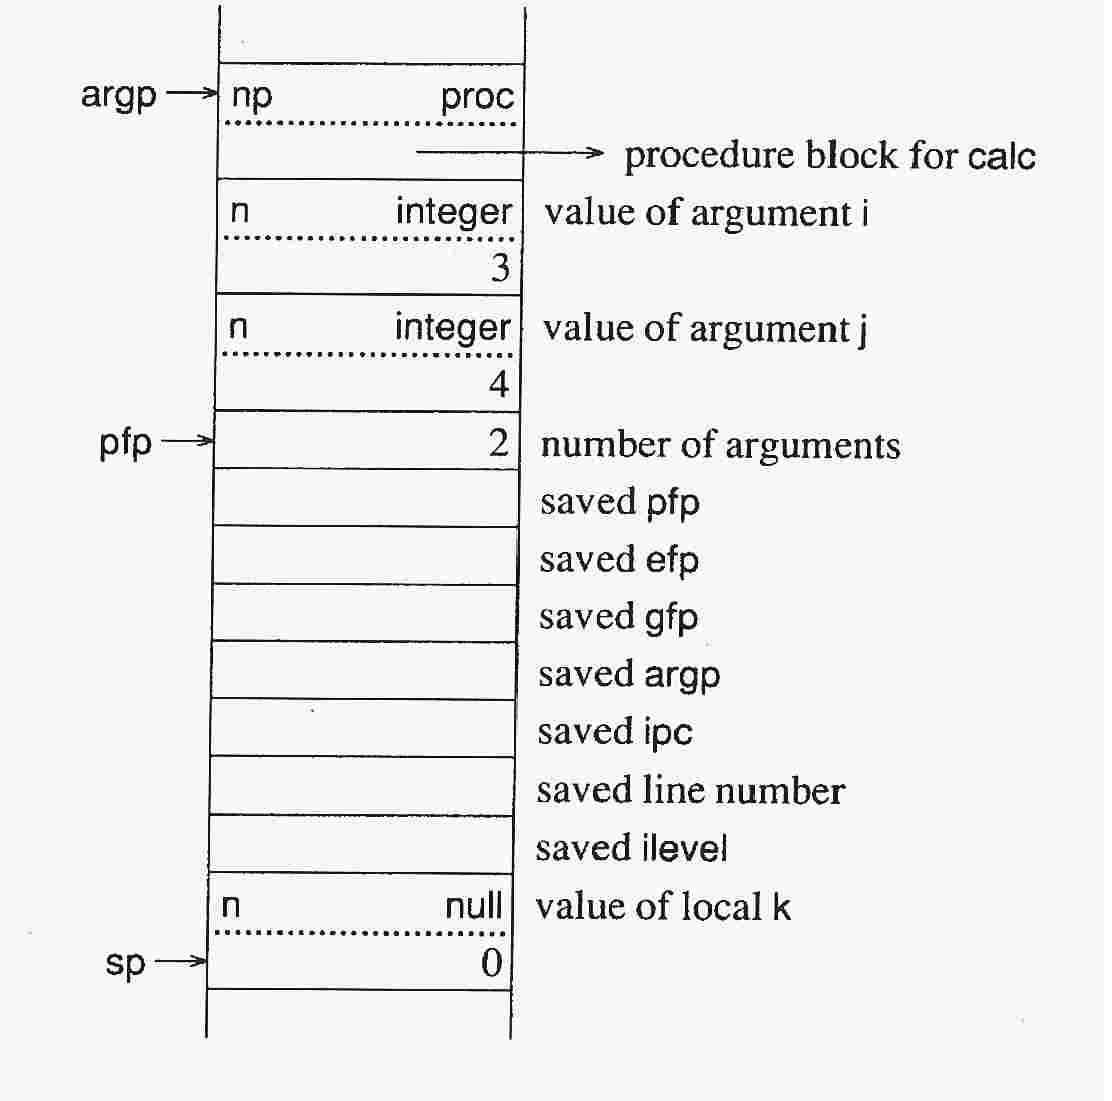
\includegraphics[width=3.7402in,height=3.6772in]{ib-img/ib-img085.jpg} 
\begin{picture}(300,300)(0,-16)
\put(100,0){\downbars}
\put(100,0){\dvbox{null}{n}{0}}
\put(100,0){\lregptr{sp}{20}}
\put(100,0){\trboxlabel{value of local k}}
\begin{picture}(0,0)(0,-32)
\put(100,0){\blkbox{}{}}
\put(100,0){\rightboxlabels{saved line number}{saved ilevel}}
\put(100,32){\blkbox{}{}}
\put(100,32){\rightboxlabels{saved argp}{saved ipc}}
\put(100,64){\blkbox{}{}}
\put(100,64){\rightboxlabels{saved efp}{saved gfp}}
\put(100,96){\blkbox{2}{}}
\put(100,96){\rightboxlabels{number of arguments}{saved pfp}}
\put(100,112){\lregptr{pfp}{20}}
\end{picture}
\put(100,160){\dvbox{integer}{n}{4}}
\put(100,160){\trboxlabel{value of argument j}}
\put(100,192){\dvbox{integer}{n}{3}}
\put(100,192){\trboxlabel{value of argument i}}
\put(100,224){\dvptrbox{proc}{np}{40}{procedure block for calc}}
\put(100,240){\lregptr{argp}{20}}
\put(100,224){\upetc}
\end{picture}

Once the null values for the local identifiers are pushed,
\texttt{ipc} is set to the entry point given in the procedure block
and \texttt{efp} and \texttt{gfp} are set to zero. Execution then
continues in the interpreter with the new \texttt{ipc}.

The three forms of return from a procedure are the same as those from
a function and correspond to the source-language expressions

%-% {\ttfamily\mdseries
%-% \ \ \ return e}
%-% 
%-% {\ttfamily\mdseries
%-% \ \ \ fail}
%-% 
%-% {\ttfamily\mdseries
%-% \ \ \ suspend e}
\goodbreak
\iconcode{
\>return e\\
\>fail\\
\>suspend e
}

The corresponding virtual machine instructions are \texttt{pret},
\texttt{pfail}, and \texttt{psusp}. For example, the virtual machine
code for

%-% {\ttfamily\mdseries
%-% \ \ \ return \&null}
\iconline{ \>return \&null }

\noindent is

%-% {\ttfamily\mdseries
%-% \ \ \ pnull}
%-% 
%-% {\ttfamily\mdseries
%-% \ \ \ pret}
\goodbreak
\iconcode{
\>pnull\\
\>pret
}

In the case of \texttt{pret}, the result currently on the top of the
interpreter stack is copied on top of the descriptor pointed to by
\texttt{argp}. If this result is a variable that is on the stack (and
hence local to the current procedure call), it is dereferenced in
place. The C stack is unwound, since there may be suspended generators
at the time of the return. The values saved in the procedure frame
marker are restored, and execution continues in the interpreter with
the restored \texttt{ipc}.

In the case of failure, the C stack is unwound as it is for
\texttt{pret}, values arc restored from the procedure frame marker,
and control is transferred to \texttt{efail}.

Procedure suspension is similar to other forms of suspension. The
descriptor on the top of the interpreter stack is dereferenced, if
necessary, and saved. A generator frame marker is constructed on the
interpreter stack to preserve values that may be needed if the
procedure call is resumed. For procedure suspension, a generator frame
marker contains two words in addition to those needed for other kinds
of generator frame markers and has the form

%--%\ \  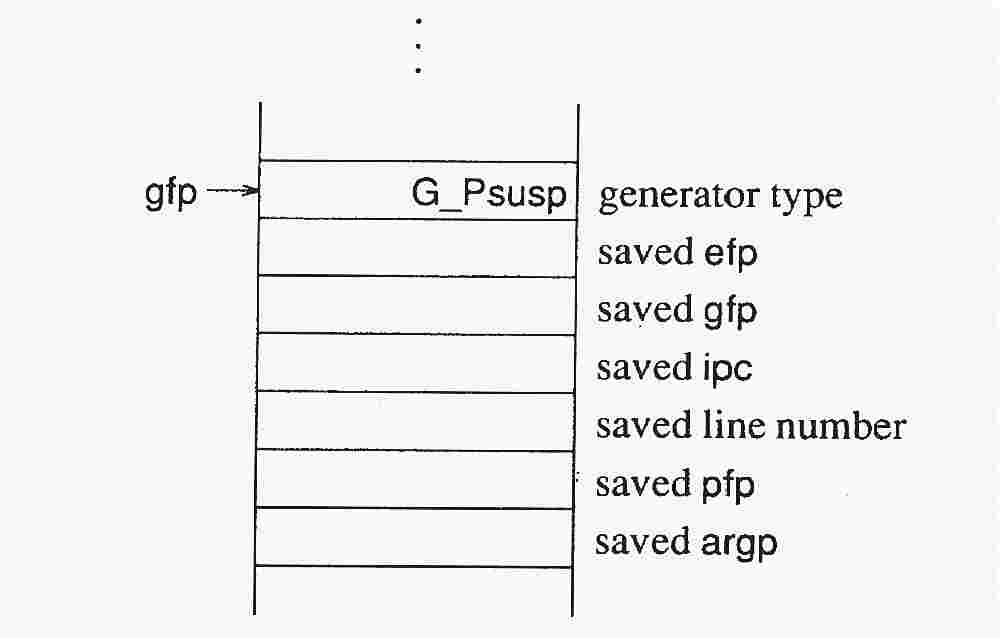
\includegraphics[width=3.6098in,height=2.2835in]{ib-img/ib-img086.jpg} 
\begin{picture}(300,160)(0,-16)
\put(100,0){\downbars}
\put(100,0){\blkbox{}{}}
\put(100,0){\rightboxlabels{saved pfp}{saved argp}}
\put(100,32){\blkbox{}{}}
\put(100,32){\rightboxlabels{saved ipc}{saved line number}}
\put(100,64){\blkbox{}{}}
\put(100,64){\rightboxlabels{saved efp}{saved gfp}}
\put(100,96){\wordbox{G\_Psusp}{}}
\put(100,96){\brboxlabel{generator type}}
\put(100,80){\upetc}
\end{picture}

After the generator frame marker is pushed, the portion of the stack
between the last generator or expression frame marker before the call
to this procedure and the word prior to \texttt{argp} is copied to the
top of the stack.  Finally, the saved descriptor, which is the result
produced by the procedure, is pushed on the top of the stack.
Execution then continues in the interpreter with the restored
\texttt{ipc}.

\section[10.4 Co{}-Expressions]{10.4 Co-Expressions}

Co-expressions add another dimension to expression evaluation in
Icon. The important thing to understand about co-expressions is that
Icon evaluation is always in \textit{some }co-expression. Although it
is not evident, the execution of an Icon program begins in a
co-expression, namely the value of \texttt{\&main}.

A co-expression requires both an interpreter stack and a C stack. In
the co-expression for \texttt{\&main}, the interpreter stack is
statically allocated and the C stack is the one normally used for C
execution--the {\textquotedbl}system stack{\textquotedbl} on some
computers. The creation of a new co-expression produces a new
interpreter stack and a new C stack, as well as space that is needed
to save state information. When a co-expression is activated, the
context for evaluation is changed to the stacks for the activated
co-expression. When the activation of a co-expression produces a
result, it in turn activates the co-expression that activated it,
leaving the stacks from which the return occurred in a state of
suspension. Thus, co-expression activation constitutes a simple
context switch.  In every co-expression, expression evaluation is in
some state, possibly actively executing, possibly suspended, or
possibly complete and unreachable.


The virtual machine instructions for

%-% {\ttfamily\mdseries
%-% \ \ \ create \textit{expr\TextSubscript{0}}}
\iconline{ \>create \textit{expr\TextSubscript{0}} }

are

%-% {\ttfamily\mdseries
%-% \ \ \ \ \ \ goto L3}
%-% 
%-% {\ttfamily\mdseries
%-% L1:}
%-% 
%-% {\ttfamily\mdseries
%-% \ \ \ \ \ \ pop}
%-% 
%-% {\ttfamily\mdseries
%-% \ \ \ \ \ \ mark L2}
%-% 
%-% {\ttfamily\itshape
%-% \ \ \ \ \ \ code for expr\TextSubscript{0}}
%-% 
%-% {\ttfamily\mdseries
%-% \textrm{\textit{\ \ \ \ \ \ }}\textrm{coret}}
%-% 
%-% {\ttfamily\mdseries
%-% \ \ \ \ \ \ efail}
%-% 
%-% {\ttfamily\mdseries
%-% L2:}
%-% 
%-% {\ttfamily\mdseries
%-% \ \ \ \ \ \ cofail}
%-% 
%-% {\ttfamily\mdseries
%-% \ \ \ \ \ \ goto L2}
%-% 
%-% {\ttfamily\mdseries
%-% L3:}
%-% 
%-% {\ttfamily\mdseries
%-% \ \ \ \ \ \ create\ \ L1}
\goodbreak
\iconcode{
\>\>goto\>\>\>\> L3\\
L1:\\
\>\>pop\\
\>\>mark\>\>\>\> L2\\
\>\>\textit{code for expr\TextSubscript{0}}\\
\>\>coret\\
\>\>efail\\
L2:\\
\>\>cofail\\
\>\>goto\>\>\>\> L2\\
L3:\\
\>\>create\>\>\>\>L1
}

Control goes immediately to \texttt{L3}, where the instruction create
constructs a co-expression block and returns a descriptor that points
to it. This block contains space for i-state variables, space for the
state of the C stack, an interpreter stack, and a C stack.

The code between \texttt{L1} and \texttt{L3} is not executed until the
co-expression is activated. The pop instruction following \texttt{L1}
discards the result transmitted to a co-expression on its first
activation, since there is no expression waiting to receive the result
of an initial activation. Next, an expression frame marker is created,
and the code for \textit{expr\TextSubscript{0}} is executed. If
\textit{expr\TextSubscript{0}} produces a result, \texttt{coret} is
executed to return the result to the activating expression. If the
co-expression is activated again, its execution continues with efail,
which causes any suspended generators in the code for
\textit{expr\TextSubscript{0}} to be resumed. If
\textit{expr\TextSubscript{0}} fails, the expression frame is removed
and \texttt{cofail} is executed. The \texttt{cofail} instruction is
very similar to the \texttt{coret} instruction, except that it signals
failure rather than producing a result. Note that if a co-expression
that returns by means of \texttt{cofail} is activated again, the
\texttt{cofail} instruction is executed in a loop.

A co-expression is activated by the expression

%-% {\ttfamily\mdseries
%-% \textit{\ \ \ expr1 }@ \textit{expr2}}
\iconline{ \textit{\ \ \ expr1 }@ \textit{expr2} }

\noindent for which the virtual machine code is

%-% {\itshape
%-% \ \ \ code for expr1}
%-% 
%-% {\itshape
%-% \ \ \ code for expr2}
%-% 
%-% 
%-% \ \ \ coact
\goodbreak
\iconcode{
\>\textit{code for expr1}\\
\>\textit{code for expr2}\\
\>coact\\
}

The more common form of activation,
\texttt{@}\textit{expr\TextSubscript{0}}, is just an abbreviation for
\makebox{\texttt{\&null @} \textit{expr\TextSubscript{0}}}; a result is always
transmitted, even if it is the null value.

The virtual machine code for \textit{expr\TextSubscript{1}} produces
the descriptor for the result that is to be transmitted to the
co-expression being activated. The \texttt{coact} instruction
dereferences the result produced by \textit{expr\TextSubscript{2}}, if
necessary, and checks to make sure it is a co-expression. After
setting up state information, \texttt{coact} transfers control to the
new co-expression with \texttt{ipc} set to \texttt{L1}. Execution
continues there. If \texttt{coret} is reached, control is restored to
the activating co-expression. The instructions \texttt{coact} and
\texttt{coret} are very similar. Each saves the current co-expression
state, sets up the new co-expression state, and transfers control.

\textbf{Co-Expression Blocks.} There is quite a bit of information
associated with a co-expression, and space is provided for it in a
co-expression block:


%--%\clearpage
%--%\ \  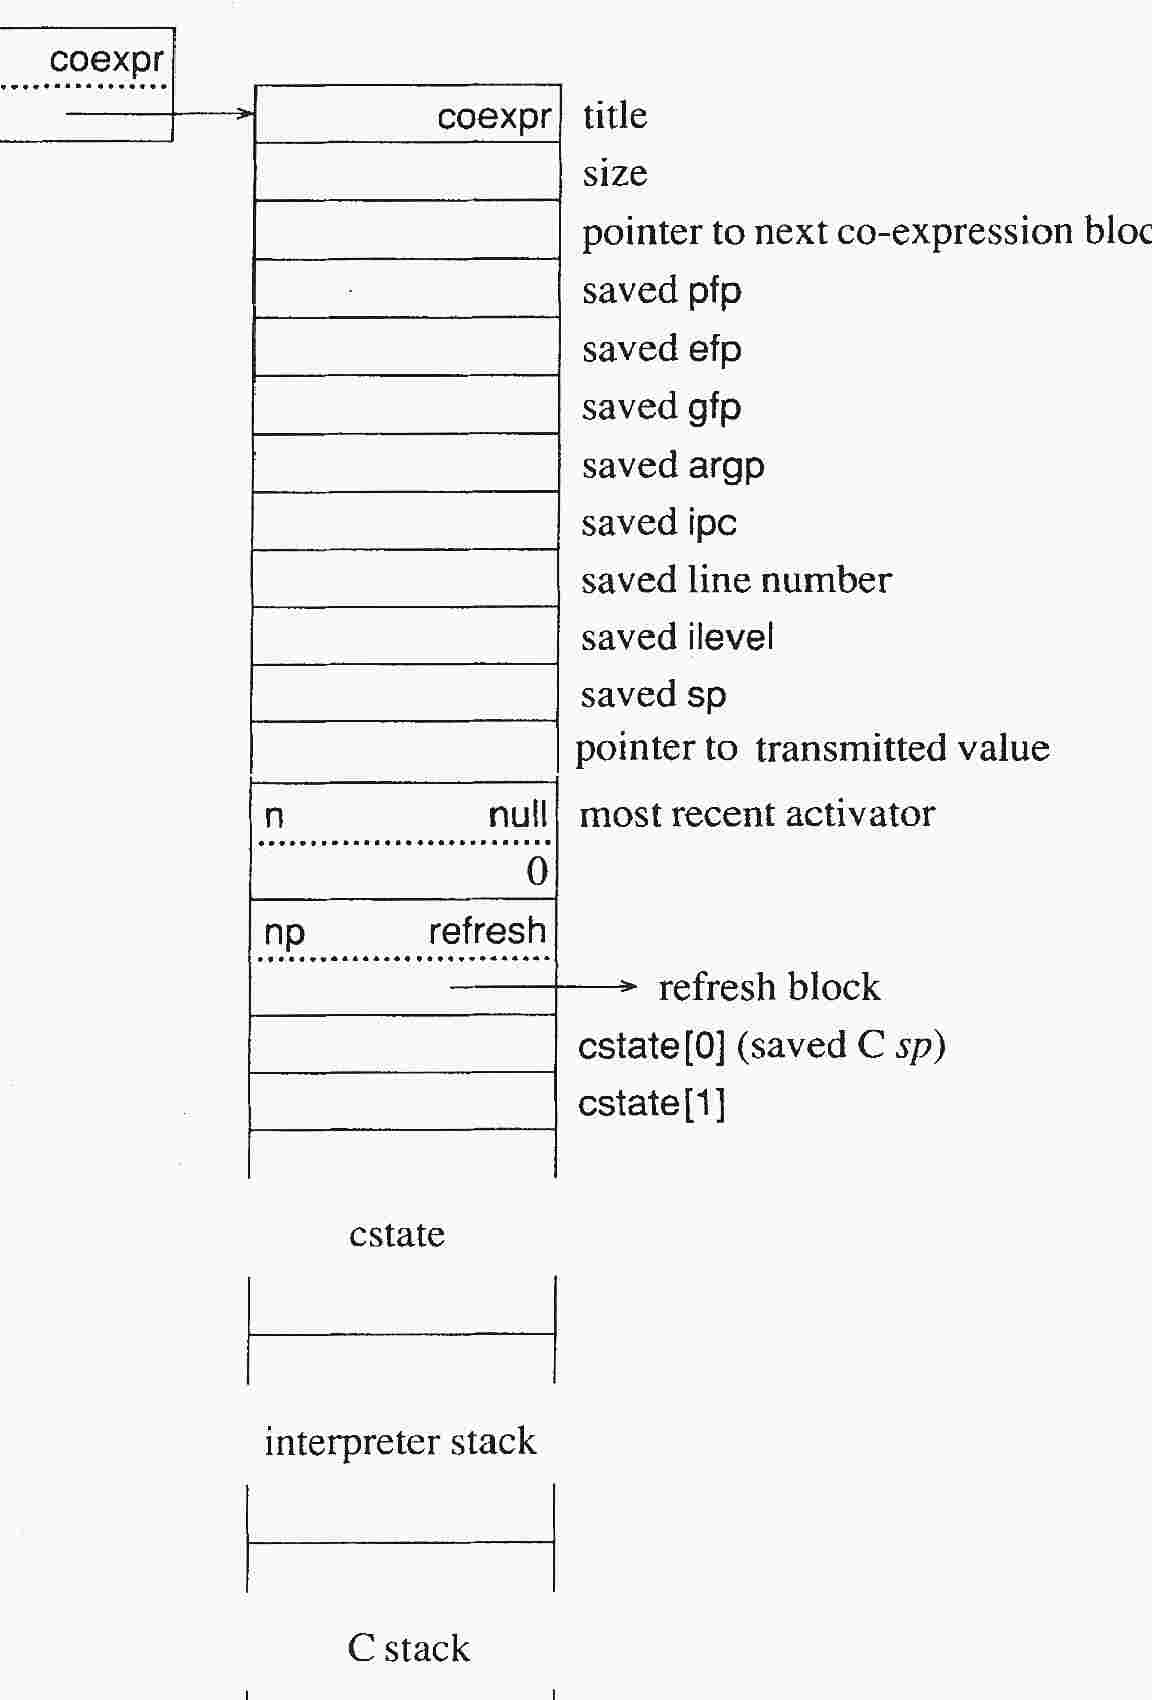
\includegraphics[width=3.9543in,height=5.678in]{ib-img/ib-img087.jpg} 
\begin{picture}(300,440)
\put(104,10){\makebox[100pt]{C stack}}
\put(100,32){\updownbars}
\put(104,52){\makebox[100pt]{interpreter stack}}
\put(100,80){\updownbars}
\put(104,100){\makebox[100pt]{cstate}}
\put(100,136){\downbars}
\put(100,136){\blkbox{}{}}
\put(100,136){\rightboxlabels{cstate[0] (saved C {\em sp})}{cstate[1]}}
\put(100,168){\dvptrbox{refresh}{np}{40}{refresh block}}
\put(100,200){\dvbox{null}{n}{0}}
\put(100,200){\trboxlabel{most recent activator}}
\put(100,232){\blkbox{}{}}
\put(100,232){\rightboxlabels{saved sp}{pointer to transmitted value}}
\put(100,264){\blkbox{}{}}
\put(100,264){\rightboxlabels{saved line number}{saved ilevel}}
\put(100,296){\blkbox{}{}}
\put(100,296){\rightboxlabels{saved argp}{saved ipc}}
\put(100,328){\blkbox{}{}}
\put(100,328){\rightboxlabels{saved efp}{saved gfp}}
\put(100,360){\blkbox{}{}}
\put(100,360){\rightboxlabels{pointer to next co-expression block}{saved pfp}}
\put(100,392){\blkbox{coexpr}{}}
\put(100,392){\rightboxlabels{title}{size}}
\put(-20,408){\dvptrbox{coexpr}{np}{40}{}}
\end{picture}

The interpreter stack and C stack shown in this diagram are not to
scale compared with the rest of the block. Both are comparatively
large; the actual sizes depend on the address space of the target
computer.


The first word of the block is the usual title. The next word contains
the number of results the co-expression has produced-its
{\textquotedbl}size.{\textquotedbl} Then there is a pointer to the
next co-expression block on a list that is maintained for garbage
collection purposes. See Sec. 11.3.4. Following this pointer there are
i-state variables: \texttt{pfp}, \texttt{efp}, \texttt{gfp},
\texttt{argp}, \texttt{ipc}, \texttt{sp}, the current program line
number, and \texttt{ilevel}.

Then there is a descriptor for the transmitted result, followed by two
more descriptors: one for the co-expression that activates this one
and one for a \textit{refresh} block that is needed if a copy of this
co-expression block is needed.  C state information is contained in an
array of words, \texttt{cstate}, for registers and possibly other
state information. The array \texttt{cstate} typically contains
fifteen words for such information. The C \textit{sp} is stored in
\texttt{cstate[0]}. The use of the rest of \texttt{cstate} is
machine-dependent.

Finally, there is an interpreter stack and a C stack. On a computer
with a downward-growing C stack, such as the VAX, the base of the C
stack is at the end of the co-expression block and the interpreter and
C stacks grow toward each other. On a computer with an upward-growing
C stack, the C stack base follows the end of the interpreter stack.

\textbf{Stack Initialization.} When a co-expression is first
activated, its interpreter stack must be in an appropriate state. This
initialization is done when the co-expression block is created. A
procedure frame, which is a copy of the procedure frame for the
procedure in which the create instruction is executed, is placed on
the new stack. It consists of the words from \texttt{argp} through the
procedure frame marker and the descriptors for the local
identifiers. The \texttt{efp} and \texttt{gfp} in the co-expression
block are set to zero and the \texttt{ipc} is set to the value given
in the argument to the \texttt{create} instruction (\texttt{L1}).

No C state is set up on the new C stack; this is handled when the
co-expression is activated the first time. The initial null value for
the activator indicates the absence of a valid C state.


\textbf{Co-Expression Activation.} As mentioned previously,
\texttt{coact} and \texttt{coret} perform many similar functions--both
save current state information, establish new state information, and
activate another co-expression.  The current i-state variables are
saved in the current co-expression block, and new ones are established
from the co-expression block for the co-expression being
activated. Similar actions are taken for the C state. Since the C
state is machine-dependent, the {\textquotedbl}context
switch{\textquotedbl} for the C state is performed by a routine,
called \texttt{coswitch()}, that contains assembly-language code.

The C state typically consists of registers that are used to address
the C stack and registers that must be preserved across the call of a
C function. On the VAX, for example, the C stack registers are
\textit{sp, ap, and fp}. Only the registers \texttt{r6} through
\texttt{r11} must be saved for some C compilers, while other C
compilers require that \texttt{r3} through \texttt{r11} be saved. Once
the necessary registers are saved in the \texttt{cstate} array of the
current co-expression, new values of these registers are
established. If the co-expression being activated has been activated
before, the C state is set up from its \texttt{cstate} array, and
\texttt{coswitch()} returns to \texttt{interp()}. At this point,
execution continues in the newly activated co-expression. Control is
transferred to the beginning of the interpreter loop, and the next
instruction (from the \texttt{ipc} for the co-expression) is fetched.

However, when a co-expression is activated for the first time, there
are no register values to restore, since no C function has yet been
called for the new co-expression. This is indicated, as mentioned
previously, by a null activator, which is communicated to
\texttt{coswitch()} by an integer argument. In this case,
\texttt{coswitch()} sets up registers for the call of a C function and
calls \texttt{interp()} to start the execution of the new
co-expression.  Such a call to \texttt{interp()} on the first
activation of a co-expression corresponds to the call to
\texttt{interp()} that starts program execution in the co-expression
\texttt{\&main} for the main procedure. There can never be a return
from the call to \texttt{interp()} made in \texttt{coswitch()}, since
program execution can only terminate normally by a return from the
main procedure, in \texttt{\&main}.

The function \texttt{coswitch()} is fastest if it is
machine-dependent. The version for the x86 with the GCC compiler is an
example:

%-% {\ttfamily\mdseries
%-% coswitch:}
%-% 
%-% {\ttfamily\mdseries
%-% \ \ pushl \%ebp}
%-% 
%-% {\ttfamily\mdseries
%-% \ \ movl \%esp,\%ebp}
%-% 
%-% {\ttfamily\mdseries
%-% \ \ movl 8(\%ebp),\%eax}
%-% 
%-% {\ttfamily\mdseries
%-% \ \ movl \%esp,0(\%eax)}
%-% 
%-% {\ttfamily\mdseries
%-% \ \ movl \%ebp,4(\%eax)}
%-% 
%-% {\ttfamily\mdseries
%-% \ \ movl 12(\%ebp),\%eax}
%-% 
%-% {\ttfamily\mdseries
%-% \ \ cmpl \$0,16(\%ebp)}
%-% 
%-% {\ttfamily\mdseries
%-% \ \ movl 0(\%eax),\%esp}
%-% 
%-% {\ttfamily\mdseries
%-% \ \ je .L2}
%-% 
%-% 
%-% \bigskip
%-% 
%-% {\ttfamily\mdseries
%-% \ \ movl 4(\%eax),\%ebp}
%-% 
%-% {\ttfamily\mdseries
%-% \ \ jmp .L1}
%-% 
%-% 
%-% \bigskip
%-% 
%-% {\ttfamily\mdseries
%-% .L2:}
%-% 
%-% {\ttfamily\mdseries
%-% \ \ movl \$0,\%ebp}
%-% 
%-% {\ttfamily\mdseries
%-% \ \ pushl \$0}
%-% 
%-% {\ttfamily\mdseries
%-% \ \ pushl \$0}
%-% 
%-% {\ttfamily\mdseries
%-% \ \ call new\_context}
%-% 
%-% {\ttfamily\mdseries
%-% \ \ pushl \$.LC0}
%-% 
%-% {\ttfamily\mdseries
%-% \ \ call syserr}
%-% 
%-% {\ttfamily\mdseries
%-% \ \ addl \$12,\%esp}
%-% 
%-% 
%-% \bigskip
%-% 
%-% {\ttfamily\mdseries
%-% .L1:}
%-% 
%-% {\ttfamily\mdseries
%-% \ \ leave}
%-% 
%-% {\ttfamily\mdseries
%-% \ \ ret}
\goodbreak
\iconcode{
coswitch:\\
\>pushl\>\> \%ebp\\
\>movl\>\> \%esp,\%ebp\\
\>movl\>\> 8(\%ebp),\%eax\\
\>movl\>\> \%esp,0(\%eax)\\
\>movl\>\> \%ebp,4(\%eax)\\
\>movl\>\> 12(\%ebp),\%eax\\
\>cmpl\>\> \$0,16(\%ebp)\\
\>movl\>\> 0(\%eax),\%esp\\
\>je\>\> .L2\\
\\
\>movl\>\> 4(\%eax),\%ebp\\
\>jmp\>\> .L1\\
\\
.L2:\\
\>movl\>\> \$0,\%ebp\\
\>pushl\>\> \$0\\
\>pushl\>\> \$0\\
\>call\>\> new\_context\\
\>pushl\>\> \$.LC0\\
\>call\>\> syserr\\
\>addl\>\> \$12,\%esp\\
\\
.L1:\\
\>leave\\
\>ret
}

If no assembler co-expression switch is available, modern platforms
with POSIX threads can use Icon 9.5.1's supported form of
co-expressions, which is more than 100x slower and approximately twice
as many lines of C. The public interface in either case looks like:

%-% {\ttfamily\mdseries
%-% int coswitch(void *old\_cs, void *new\_cs, int first);}
\iconline{ int coswitch(void *old\_cs, void *new\_cs, int first); }

The variables \texttt{old\_cs} and \texttt{new\_cs} are pointers to
the \texttt{cstate} arrays for the activating and activated
co-expressions, respectively. The value of first is 0 if the
co-expression is being activated for the first time. Note that in
order to write \texttt{coswitch()} it is necessary to know how the
first two arguments are accessed in assembly language. For the
previous example, \texttt{old\_cs} and \texttt{new\_cs} are eight and
twelve bytes from the \textit{ebp }register, respectively.

\textbf{Refreshing a Co-Expression}. The operation
\texttt{\textit{\^{}}}\textit{expr\TextSubscript{0}} creates a copy of
the co-expression produced by \textit{expr\TextSubscript{0}} with its
state initialized to what it was when it was originally created. The
refresh block for \textit{expr\TextSubscript{0}} contains the
information necessary to reproduce the initial state. The refresh
block contains the original \texttt{ipc} for the co-expression, the
number of local identifiers for the procedure in which
\textit{expr\TextSubscript{0}} was created, a copy of the procedure
frame marker at the time of creation, and the values of the arguments
and local identifiers at the time of creation. Consider, for example,

%-% {\ttfamily\mdseries
%-% \ \ \ procedure labgen(s)}
%-% 
%-% {\ttfamily\mdseries
%-% \ \ \ \ \ \ local i, j, e}
%-% 
%-% {\ttfamily\mdseries
%-% \ \ \ \ \ \ i := 1}
%-% 
%-% {\ttfamily\mdseries
%-% \ \ \ \ \ \ j := 100}
%-% 
%-% {\ttfamily\mdseries
%-% \ \ \ \ \ \ e := create (s {\textbar}{\textbar} (i to j) {\textbar}{\textbar} {\textquotedbl}:{\textquotedbl})}
%-% 
%-% {\ttfamily\mdseries
%-% \ \ \ end}
\goodbreak
\iconcode{
\>procedure labgen(s)\\
\>\>local i, j, e\\
\>\>i := 1\\
\>\>j := 100\\
\>\>e := create (s || (i to j) || ":")\\
\>end
}


For the call \texttt{labgen({\textquotedbl}L{\textquotedbl})}, the refresh block for \texttt{e} is


%--%\ \  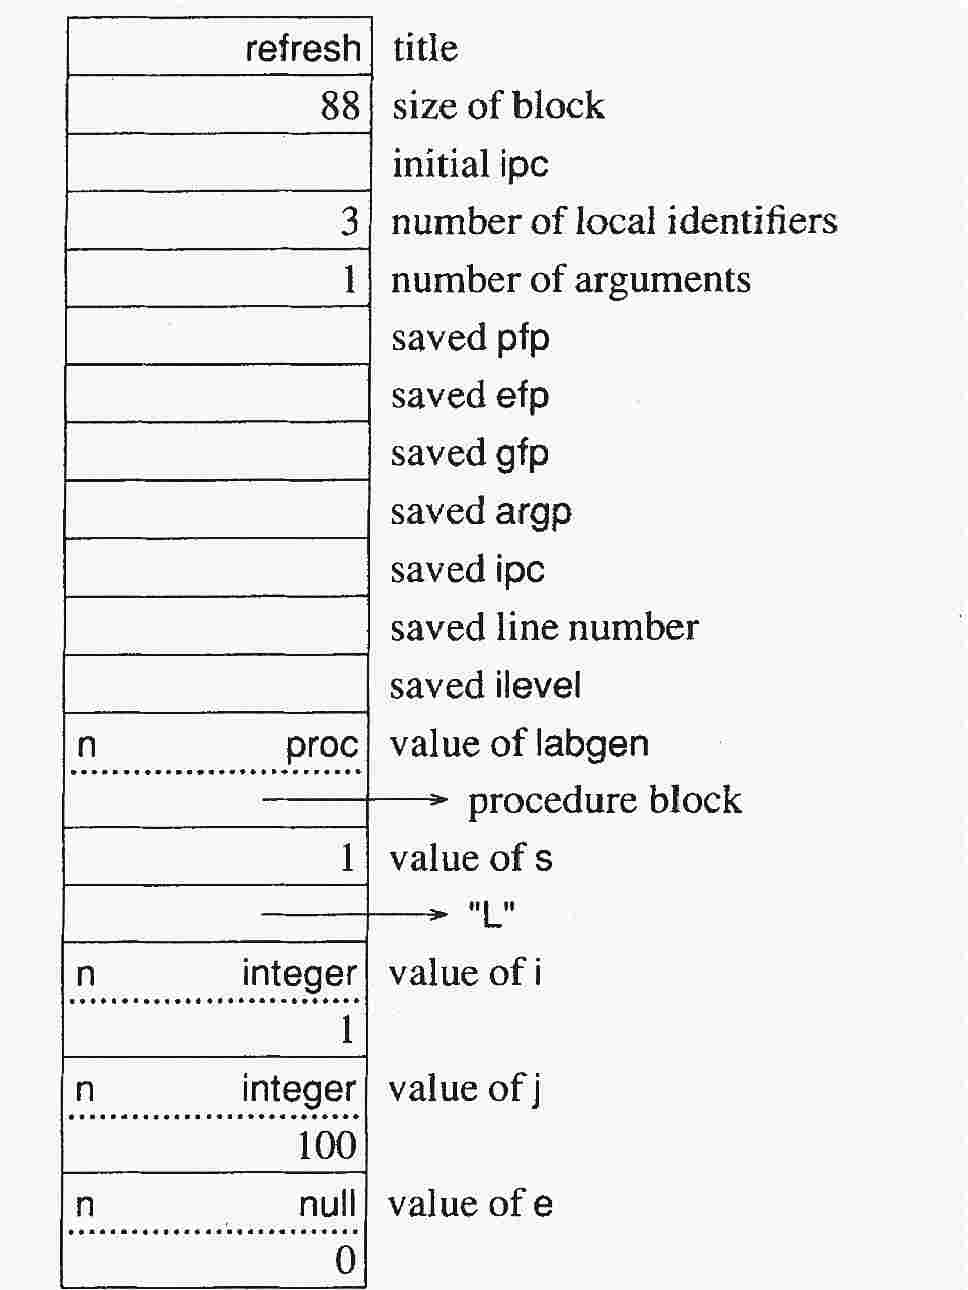
\includegraphics[width=3.3134in,height=4.3075in]{ib-img/ib-img088.jpg} 
\begin{picture}(300,380)
\put(100,0){\dvbox{null}{n}{0}}
\put(100,0){\trboxlabel{value of e}}
\put(100,32){\dvbox{integer}{n}{100}}
\put(100,32){\trboxlabel{value of j}}
\put(100,64){\dvbox{null}{n}{1}}
\put(100,64){\trboxlabel{value of i}}
\put(100,96){\dvptrbox{1}{}{40}{"L"}}
\put(100,96){\trboxlabel{value of s}}
\put(100,128){\dvptrbox{proc}{n}{40}{procedure block}}
\put(100,128){\trboxlabel{value of labgen}}
\put(100,160){\blkbox{}{}}
\put(100,160){\rightboxlabels{saved line number}{saved ilevel}}
\put(100,192){\blkbox{}{}}
\put(100,192){\rightboxlabels{saved argp}{saved ipc}}
\put(100,224){\blkbox{}{}}
\put(100,224){\rightboxlabels{saved efp}{saved gfp}}
\put(100,256){\blkbox{}{}}
\put(100,256){\rightboxlabels{saved number of arguments}{saved pfp}}
\put(100,288){\blkbox{}{3}}
\put(100,288){\rightboxlabels{initial ipc}{number of local identifiers}}
\put(100,320){\blkbox{refresh}{88}}
\put(100,320){\rightboxlabels{title}{size of block}}
\end{picture}

\textsc{Retrospective}: Invocation expressions are more complicated to
implement than operators, since the meaning of an invocation
expression is not known until it is evaluated. Since functions and
procedures are source-language values, the information associated with
them is stored in blocks in the same manner as for other types.

The C code that implements Icon functions is written in the same
fashion as the code for operators. Procedures have source-language
analogs of the failure and suspension mechanisms used for implementing
functions and operators.  Procedure frames identify the portions of
the interpreter stack associated with the procedures currently
invoked.

A co-expression allows an expression to be evaluated outside its
lexical site in the program by providing separate stacks for its
evaluation. The possibility of multiple stacks in various states of
evaluation introduces technical problems in the implementation,
including a machine-dependent context switch.

\bigskip

\noindent\textbf{EXERCISES}

\textbf{10.1} What happens if a call of a procedure or function
contains an extra argument expression, but the evaluation of that
expression fails?

\textbf{10.2} Sometimes it is useful to be able to specify a function
or procedure by means of its string name. Icon supports
{\textquotedbl}string invocation,{\textquotedbl} which allows the
value of \textit{expr\TextSubscript{0}} in

%-% {\ttfamily\mdseries
%-% \textit{\ \ \ expr\TextSubscript{0}(expr\TextSubscript{1},
%-% expr\TextSubscript{2}, ..., expr\TextSubscript{n})}}
\goodbreak
\iconline{
\>\textit{ expr\TextSubscript{0}(expr\TextSubscript{1},
expr\TextSubscript{2}, ..., expr\TextSubscript{n})}
}

\noindent to be a string. Thus,

%-% {\ttfamily\mdseries
%-% \ \ \ {\textquotedbl}write{\textquotedbl}(s)}
\iconline{ \>"write"(s) }

\noindent produces the same result as

%-% {\ttfamily\mdseries
%-% \ \ \ write(s)}
\iconline{ \>write(s) }

Of course, such a string name is usually computed, as in

%-% {\ttfamily\mdseries
%-% \ \ \ (read())(s)}
\iconline{ \>(read())(s) }

Describe what is involved in implementing this aspect of
invocation. Operators also may be invoked by their string names, as in

%-% {\ttfamily\mdseries
%-% \ \ \ {\textquotedbl}+{\textquotedbl}(i,j)}
\iconline{ \>"+"(i,j) }

What is needed in the implementation to support this facility? Can a
control structure be invoked by a string name?

\textbf{10.3} If the result returned by a procedure is a variable, it
may need to be dereferenced. This is done in the code for
\texttt{pret} and \texttt{psusp}. For example, if the result being
returned is a local identifier, it must be replaced by its value What
other kinds of variables must be dereferenced? Is there any difference
in the dereferencing done by \texttt{pret} and \texttt{psusp}?

\textbf{10.4} How is the structure of a co-expression block different
on a computer with an upward-growing C stack compared to one with a
downward-growing C stack? What is the difference between the two cases
in terms of potential storage fragmentation?
